\section{Related Work}

\begin{figure*}
	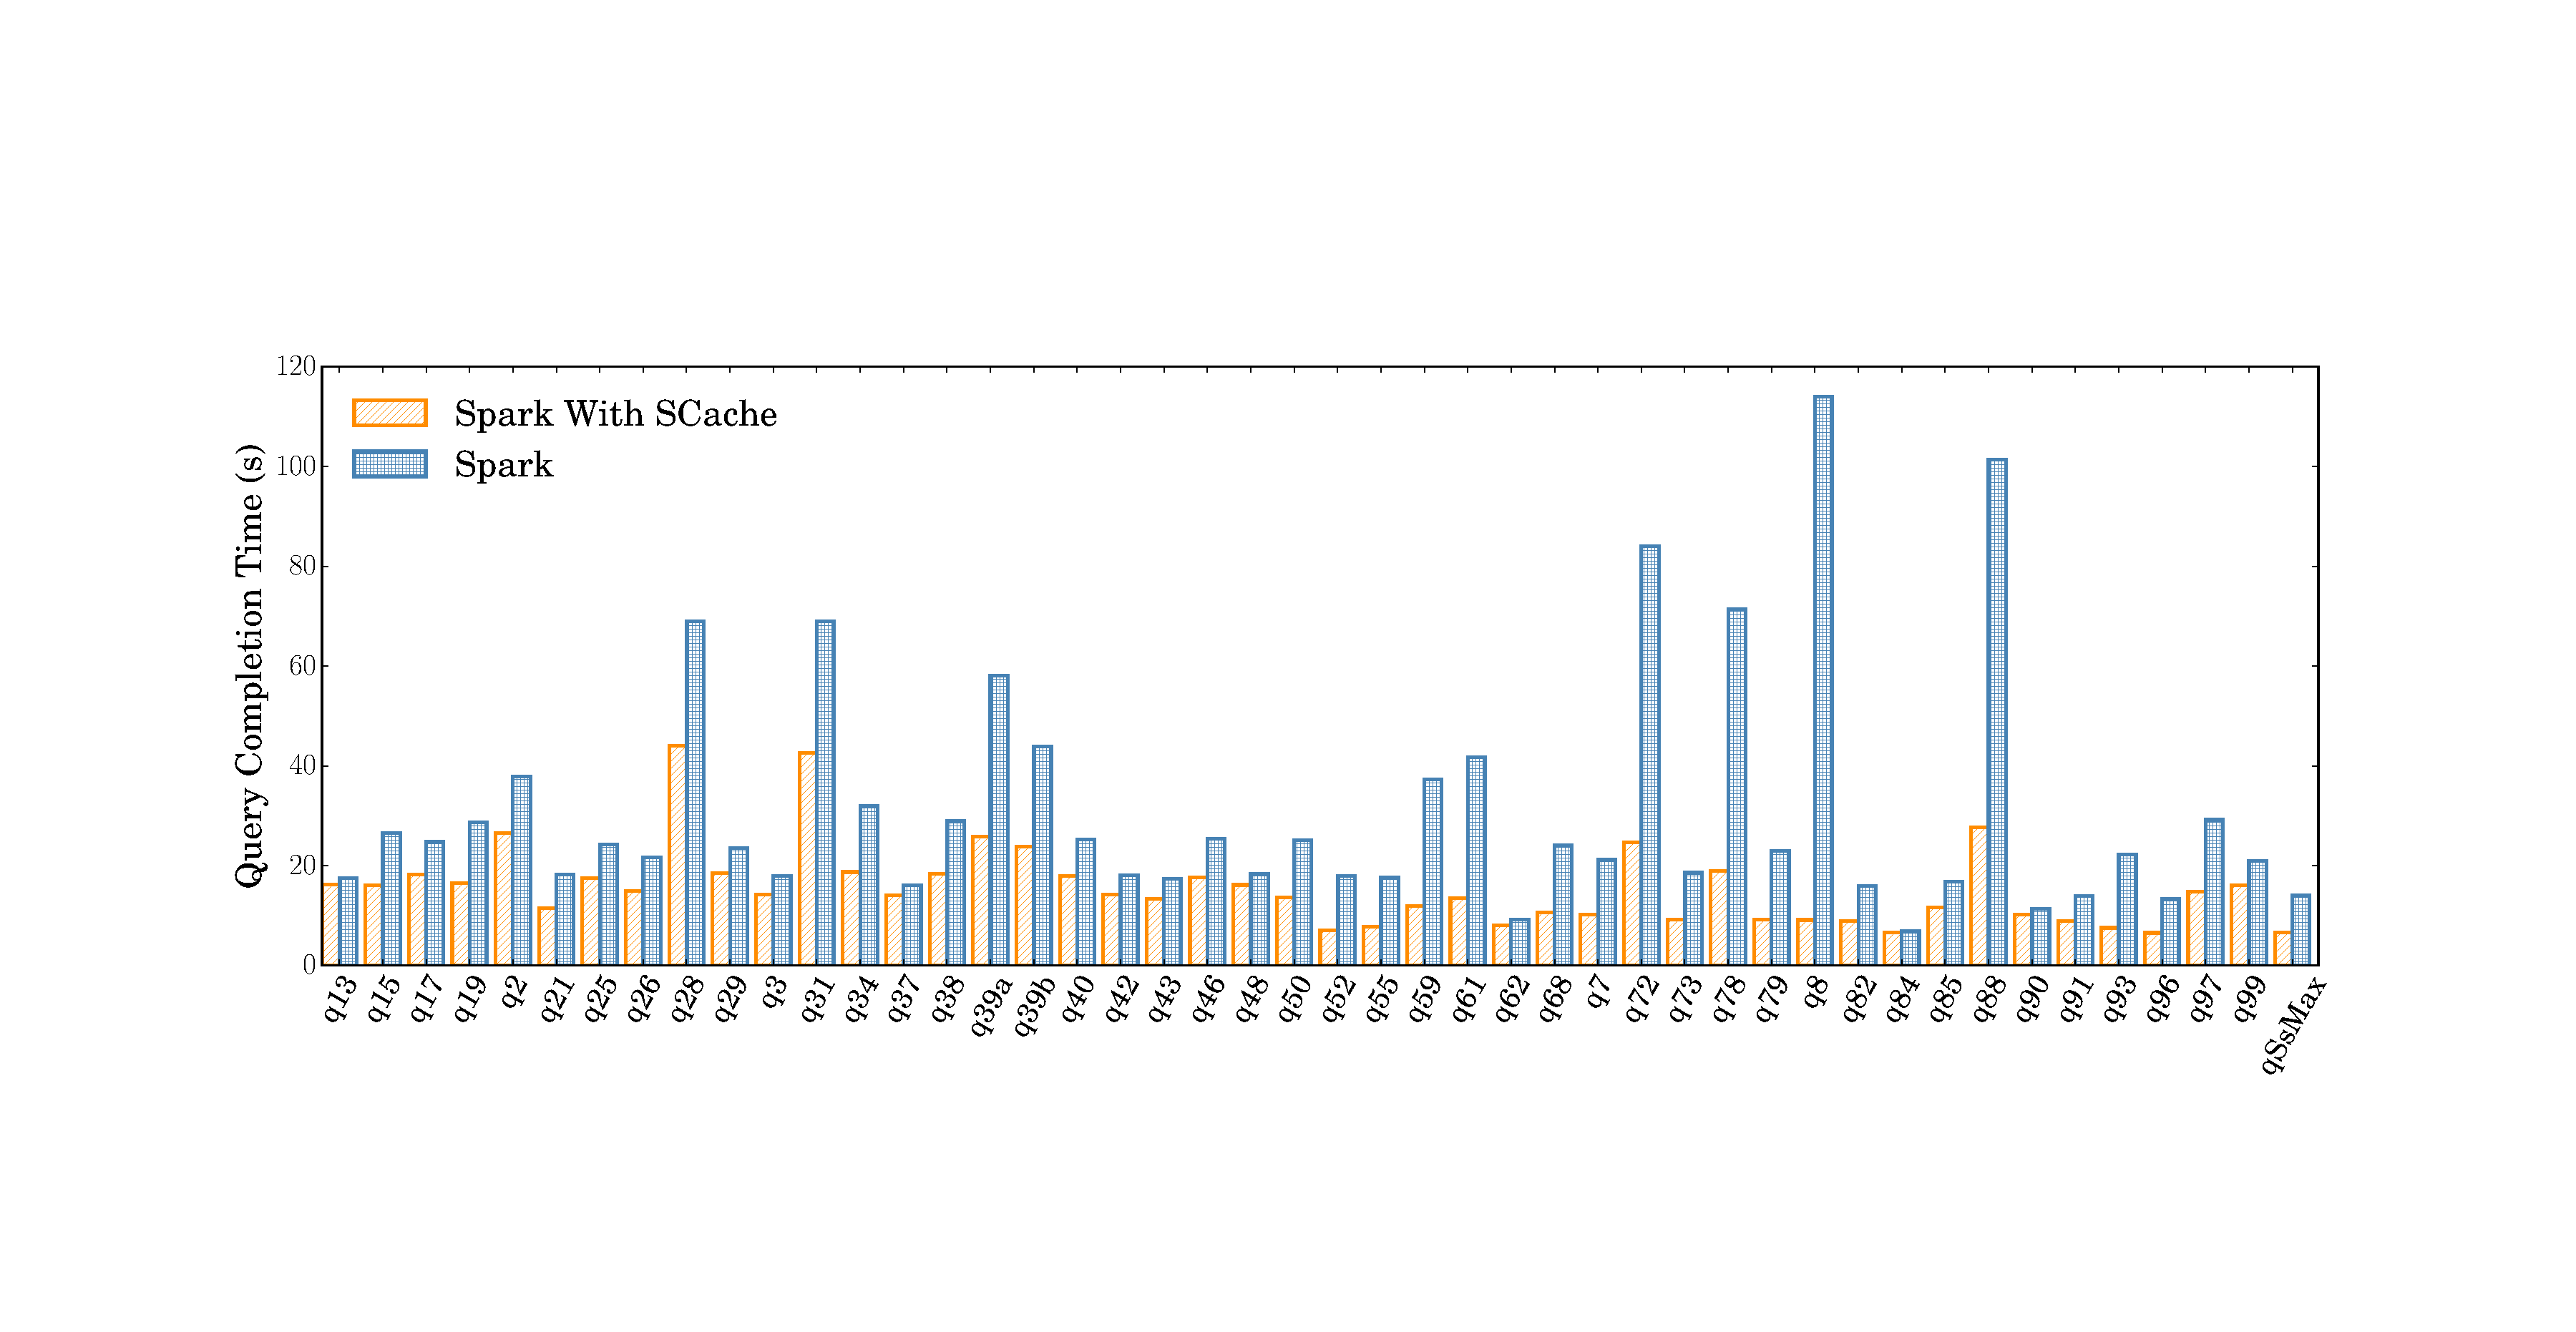
\includegraphics[width=\textwidth]{fig/tpcds}
	\caption{TPC-DS Benchmark Evaluation}
	\label{fig:tpcds}
\end{figure*}

We summarize the shuffle optimization scheduling schemes in this Section. Basically, we categorize related works in two parts, pre-scheduling and delay scheduling.

Pre-scheduling: Starfish\cite{starfish} is a self-tuning system in Hadoop. The basic idea is to get sampled data statics for tuning system parameters (e.g. slowstart, map and reduce slot ratio, etc). However, these parameters cannot be changed once the jobs begin. DynMR\cite{dynmr} dynamically starts reduce tasks in late map stage when there is enough data to be fetched. Thus it reduces the time for reducer to wait for mapper producing outputs. Those two works still left the explicit I/O time wait in both map and reduce phases. iShuffle\cite{ishuffle} decouples shuffle from reducers and designs a centralized shuffle controller. The goal is also to find the right time, but it can neither handle multiple shuffles multiple nor schedule multiple rounds of reduce tasks. iHadoop\cite{ihadoop} aggressively pre-schedules tasks in multiple successive stages, in order to start fetching data from previous stage earlier. But we have proved that randomly assign tasks may hurt the overall performance in section \ref{randomassign}. Different from these works, SCache pre-schedules reduce tasks without consuming new task slots, whereas all these schemes do.

Delay-scheduling: Delay Scheduling\cite{delay} delays tasks assignment to get better data locality, which can reduce the network traffic. ShuffleWatcher\cite{shufflewatcher} delays shuffle fetching when network is saturated. At the same time, it achieves better data locality. Both Quincy\cite{quincy} and Fair Scheduling\cite{preemptive} can reduce shuffle data by optimizing data locality of map tasks.Even though these kind of schemes can achieve higher data locality, they cannot breach the shuffle cut off between map and reduce stages, whereas SCache does. 